\subsubsection{Employer Branding}\label{employer_branding}
%Philipp


The \textit{employerBranding} (\gls{eB}) is the score which is reported to the external world in order to measure the value of the company as an employer in total. This score is comparable to the total score for companies which is presented on websites like kununu or glassdoor. The \textit{employerBranding} is a combined score out of the \textit{totalJobSatisfaction} (\gls{tJS}) and the \textit{companyImage}. As the \textit{companyImage} implicitly incluences the \textit{totalJobSatisfaction} it is weighted with 0.4 in the calculation of the \textit{employerBranding}. Formula \ref{employer_branding_general} shows how the \textit{employerBranding} is calculated in general.
\begin{equation}
    eB = 0.4 \cdot cIS + 0.6 \cdot tJS
    \label{employer_branding_general}
\end{equation}

In order to make the \textit{employerBranding} rating more realistic, we need to think about extreme cases where either the \textit{totalJobSatisfaction} or the \textit{companyImage} is rated very low. The usage of a simple weighted average would have the effect that values of $tJS = 100$ and $cI = 0$ lead to an overall score of 60.
Therefore we need to include an indicator function which incorporates a punishment for smaller values. How this is done in detail can be seen in the function \ref{employer_branding_detail}.

\begin{equation}
    \lceil (((0.4 \cdot cI + 0.6 \cdot tJS \cdot 
        \begin{cases}
             \frac{0.5}{10} & \text{if} \; cI < 30\\
             \frac{0.8}{10} & \text{if} \; cI < 60\\
             \frac{1}{10} & \text{otherwise} \\
        \end{cases}
    \rceil
    \label{employer_branding_detail}
\end{equation}

By this we ensure a sufficient punishment of the overall \textit{employerBranding}. 

\begin{comment} % is now explained with a mathematical formula
This can be done by incorporating a multiplier which is based on an IF statement. See the \textit{Excel} implementation below:
\begin{center}
   $=ROUND(((0.4 \cdot cI+0.6 \cdot tJS) \cdot IF(cI<30,0.5,IF(cI<60,0.8,IF(cI>60,1))))/10,0)$
\end{center}

The following pseudo code explains the statement above.
\begin{itemize}
    \item score = 0.4*CI + 0.6*tJS
    \item IF CI $\leq$ 30 THEN Employer Branding = Employer Branding * 0.5
    \item ELSEIF CI $\leq$ 60 THEN Employer Branding = Employer Branding * 0.8
    \item ELSEIF CI $\geq$ 60 THEN Employer Branding = Employer Branding * 1
\end{itemize}

% leave out the 3D figure
To achieve this we need to create a matrix and a 3D graph to visualize the possible implications on the employer branding. Graphic \ref{img:EBS} shows the implications of the two input parameters on the Employer Branding.

\begin{figure}
	\centering
	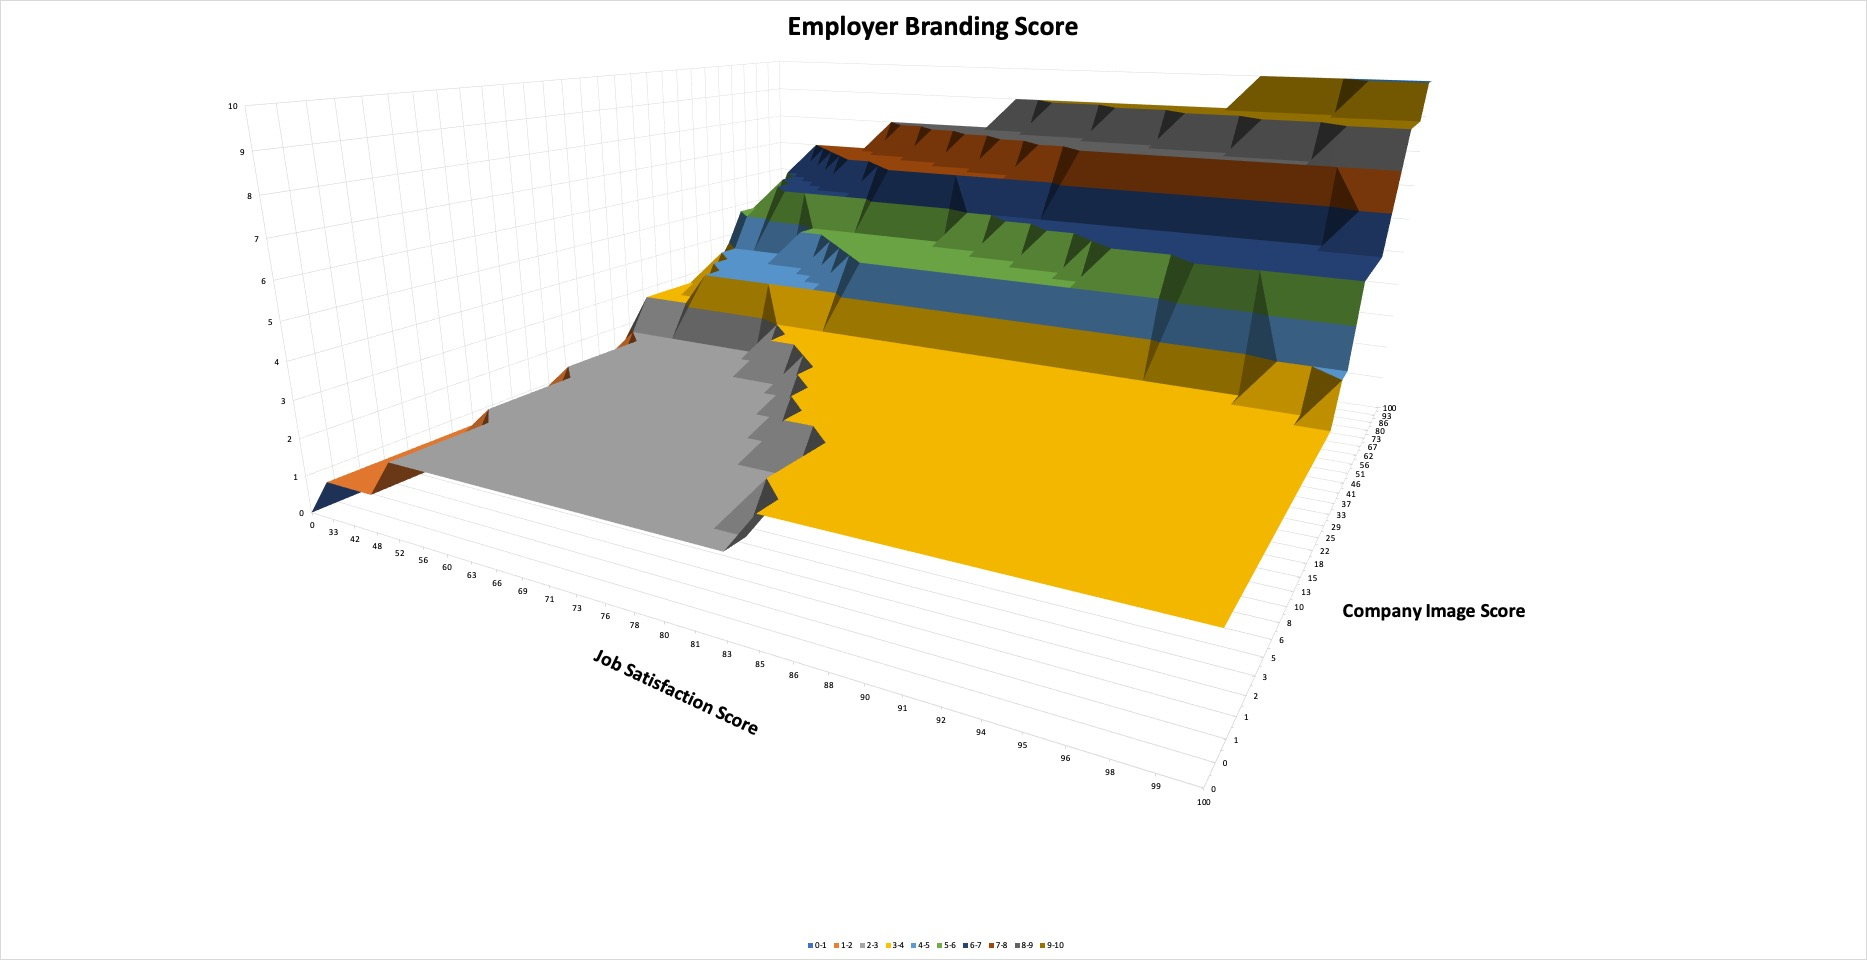
\includegraphics[width=12.5cm]{images/EBS.jpg}
	\caption{Employer Branding Score Calculation}
	\label{img:EBS}
\end{figure}
\end{comment}